\documentclass[11pt]{article}

\usepackage[a4paper,margin=0.7in]{geometry}
\usepackage[utf8]{inputenc}
\usepackage[T1]{fontenc}
\usepackage[spanish]{babel}
\usepackage{amsmath, amssymb}
\usepackage{enumitem}
\usepackage{extramarks}
\usepackage{url}
\usepackage{graphicx}
\usepackage{fancyhdr}
\usepackage[dvipsnames]{xcolor}
\geometry{a4paper}

\graphicspath{{img}}

\newcounter{problemCounter}
% \setcounter{problemCounter}{1}

\newenvironment{problem}[1][-1]{
  \ifnum#1>0
    \setcounter{problemCounter}{#1}
  \else 
    \refstepcounter{problemCounter}
  \fi
  \noindent
  \textbf{\arabic{problemCounter}) }
}{}


\title{Nivel de Aplicaciones y de
Transporte del Modelo TCP/IP}	% Titulo del trabajo.
\author{Alan Romero}			% Nombre y apellido
\newcommand{\padron}{108316}    % Padrón
\newcommand{\tpnumber}{1}       % Número de trabajo práctico
\date{\today}					% Fecha (automática, no tocar)

\makeatletter
\let\thetitle\@title
\let\theauthor\@author
\let\thedate\@date
\makeatother

% \pagestyle{fancy}
% \fancyhf{}
% \rhead{\theauthor}
% \lhead{\thetitle}
% \cfoot{\thepage}


\begin{document}
\begin{titlepage}
    
\includegraphics[scale = 0.71]{logofiuba.png}\\[.5 cm]	    % Logo fiuba
    \centering
	\textsc{\Large TB067}\\[0.2 cm]
	\textsc{\large Redes de Comunicaciones}\\[7 cm]
	\textcolor{cyan}{{\fontsize{35.83}{60}\selectfont \bfseries \thetitle}}\\[0.5cm]
	{ \Large \bfseries Trabajo Práctico N$^\circ$\tpnumber}\\[7cm]
	
	
    \noindent\makebox[\linewidth]{\rule{\textwidth}{0.4pt}}\\[0.5cm]
    \begin{minipage}{.4\textwidth}
    \textbf{Autor}:\\
	Alan Romero \\	Ezequiel
    \end{minipage}%
    \begin{minipage}{.4\textwidth}
    \textbf{Padrón}:\\
    108316 \\ XXXXXX
    \end{minipage}%
    \begin{minipage}{.2\textwidth}
    \textbf{Fecha}:\\
    \thedate \\
    \end{minipage}
	\vfill
\end{titlepage}

\section{Actividades}\label{sec:actividades} % (fold)
\begin{problem}
    Se vinculan los siguientes conceptos:
	\begin{enumerate}
        \item \textbf{gRPC}: Marco de trabajo para implementar llamadas  a procedimientos remotos.
        \item \textbf{ HTTP/2}: Protocolo de aplicación que permite  multiplexación de múltiples flujos sobre una  única conexión.
        \item \textbf{Transmission Control Protocol (TCP)}: Protocolo de transporte confiable y  full-duplex sobre el cual se establece la  conexión.
        \item \textbf{Stream}: Serialización binaria compacta definida  mediante archivos {\color{ForestGreen}\texttt{.proto}}
        \item \textbf{Channel}: Flujo independiente de datos dentro de una  conexión multiplexada.
            % Creo que Stream y Channel están al revés
        \item \textbf{Protocol Buffers}: Conexión lógica que agrupa múltiples  llamadas RPC sobre una misma conexión física.
        \item \textbf{StatusCode}: Código que indica éxito o tipo de error en una  llamada remota.
        \item \textbf{Unary RPC}: Tipo de llamada que envía un único request  y recibe una única respuesta.
        \item \textbf{Bidirectional Streaming RPC}:  Tipo de llamada donde cliente y servidor  pueden enviarse múltiples mensajes sin orden  predefinido.
        \item \textbf{Deadline}: Límite de tiempo máximo permitido para que  una llamada RPC finalice.

	\end{enumerate}
\end{problem}
% section Actividades (end)


\begin{problem}[3]
    \begin{enumerate}[label=\alph*.]
        \item La interfaz que muestra actividad con el cliente/servidor en Wireshark es Loopback/lo.
        Dadas la optimizaciones del kernel, aunque se configure un puerto e IP para la interfaz de red, el tráfico sigue yendo por loopback.

        \begin{figure}[h]
            \centering
            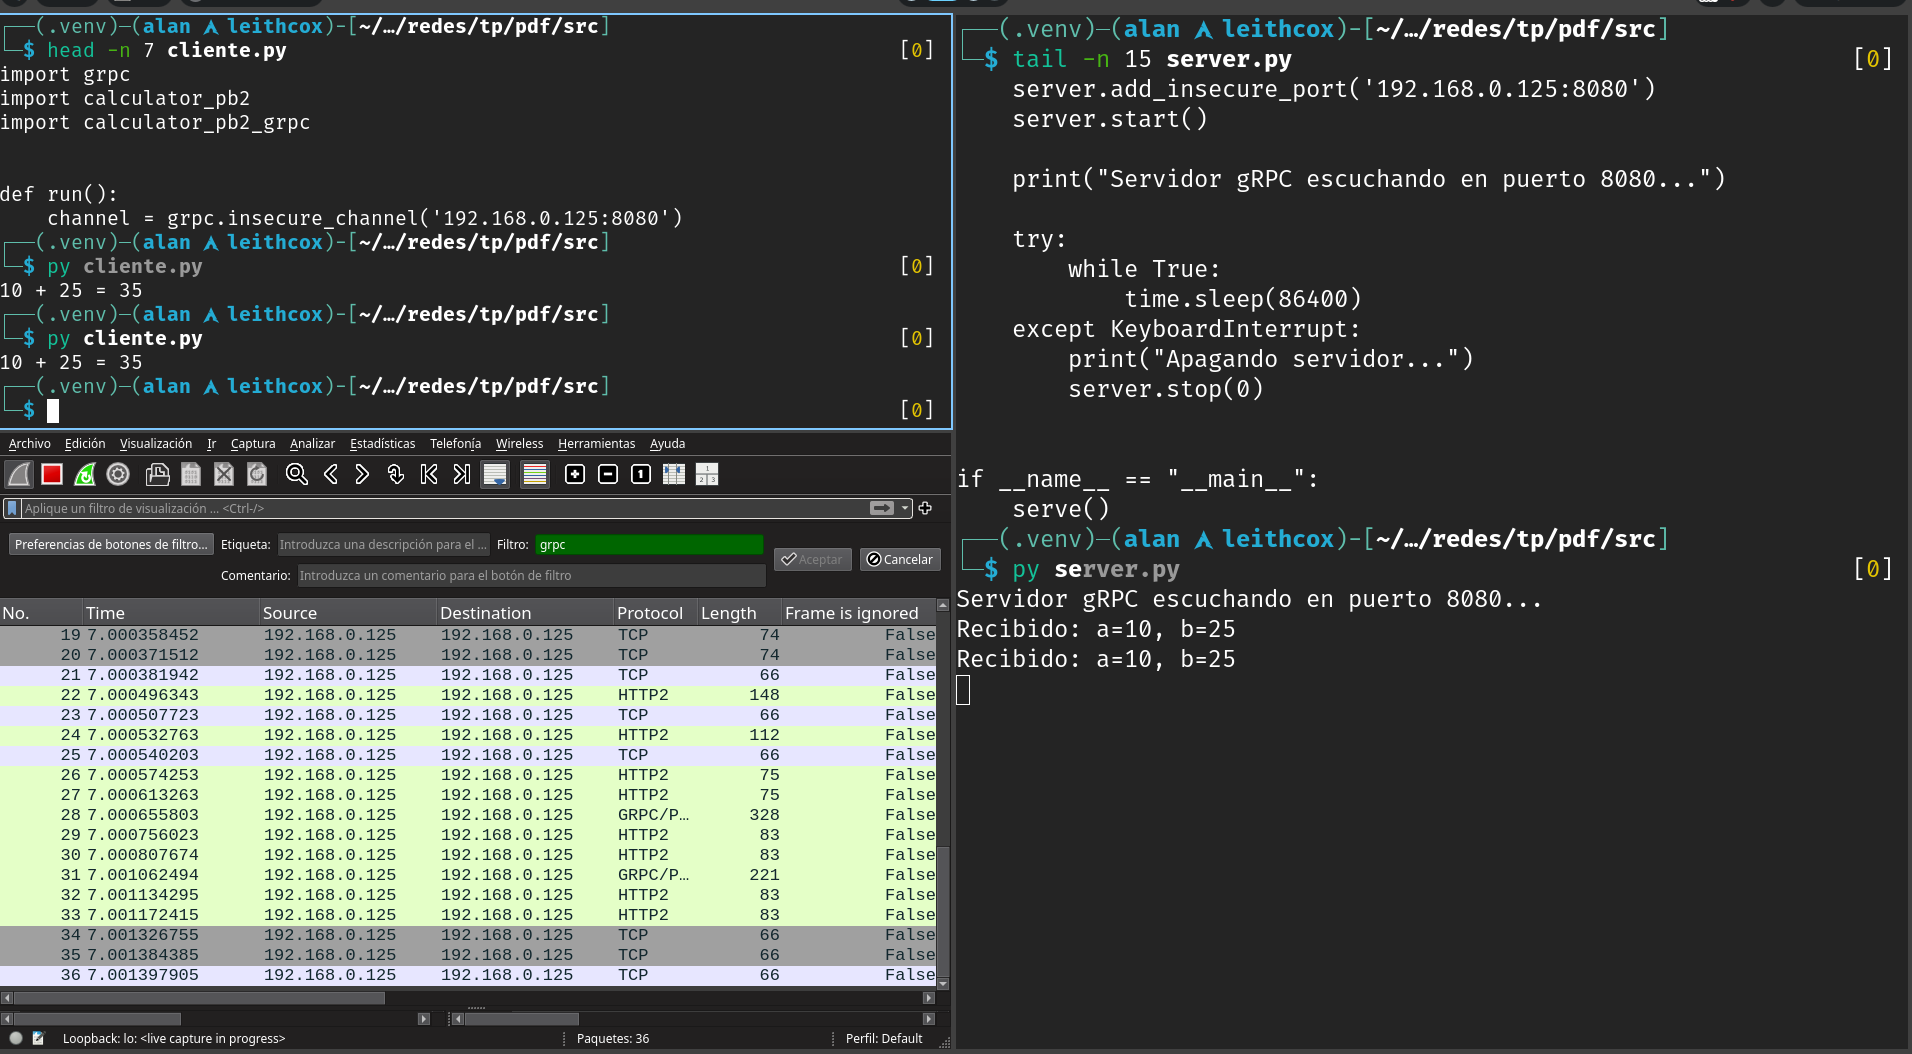
\includegraphics[width=1 \textwidth]{3a}
            \caption{Captura del tráfico en la interfaz loopback.}
            \label{fig:3a}
        \end{figure}

        Como se observa en la figura~\ref{fig:3a}, la interfaz es Loopback, aunque en el código se configuró la IP de la interfaz local WIFI.


        \item Se puede utilizar tanto IPv4 como Ipv6.
            Para realizar este ajuste, se configura al llamar a la función, pasándole por parámetro la IP en el formato de la versión que se desee.

            \begin{itemize}
                \item Para IPv4

                    \texttt{grpc.insecure\_channel('192.168.0.5:50051')}

                    \texttt{server.add\_insecure\_port('192.168.0.5:50051')}

                \item Para IPv6

                    \texttt{grpc.insecure\_channel('[::1]:50051')}

                    \texttt{server.add\_insecure\_port('[::1]:50051')}
            \end{itemize}

            \begin{figure}[h]
                \centering
                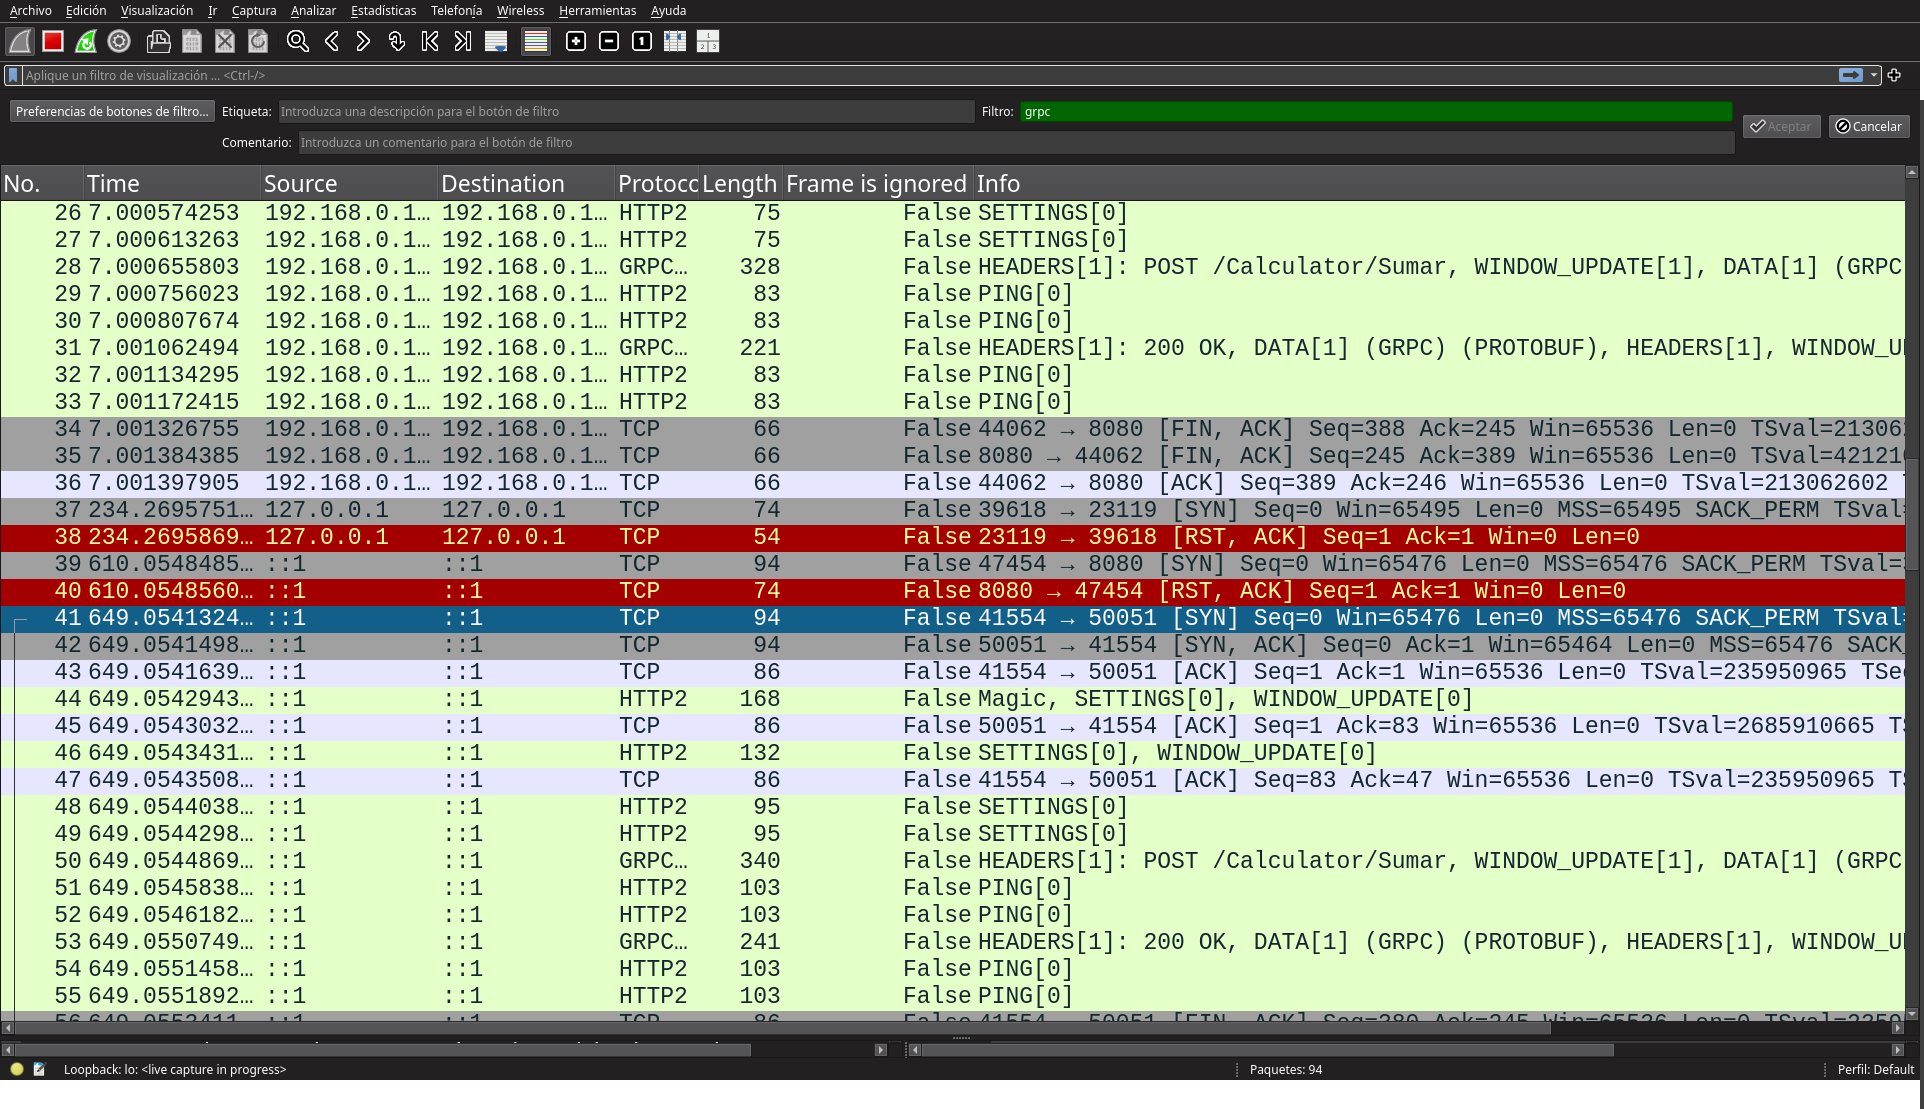
\includegraphics[width=.8 \textwidth]{3b}
                \caption{}
                \label{fig:3b}
            \end{figure}

        \item Para los ítems anteriores, se configuraron los puertos 8080 y 50051.
            No existen puertos estandar de la IANA para gRPC.

        \item Al ejecutar el servidor en varias ventanas a la vez, cuando se reciben varias peticiones de clientes, se asigna a un servidor para atender la petición.
            \begin{figure}[h]
                \centering
                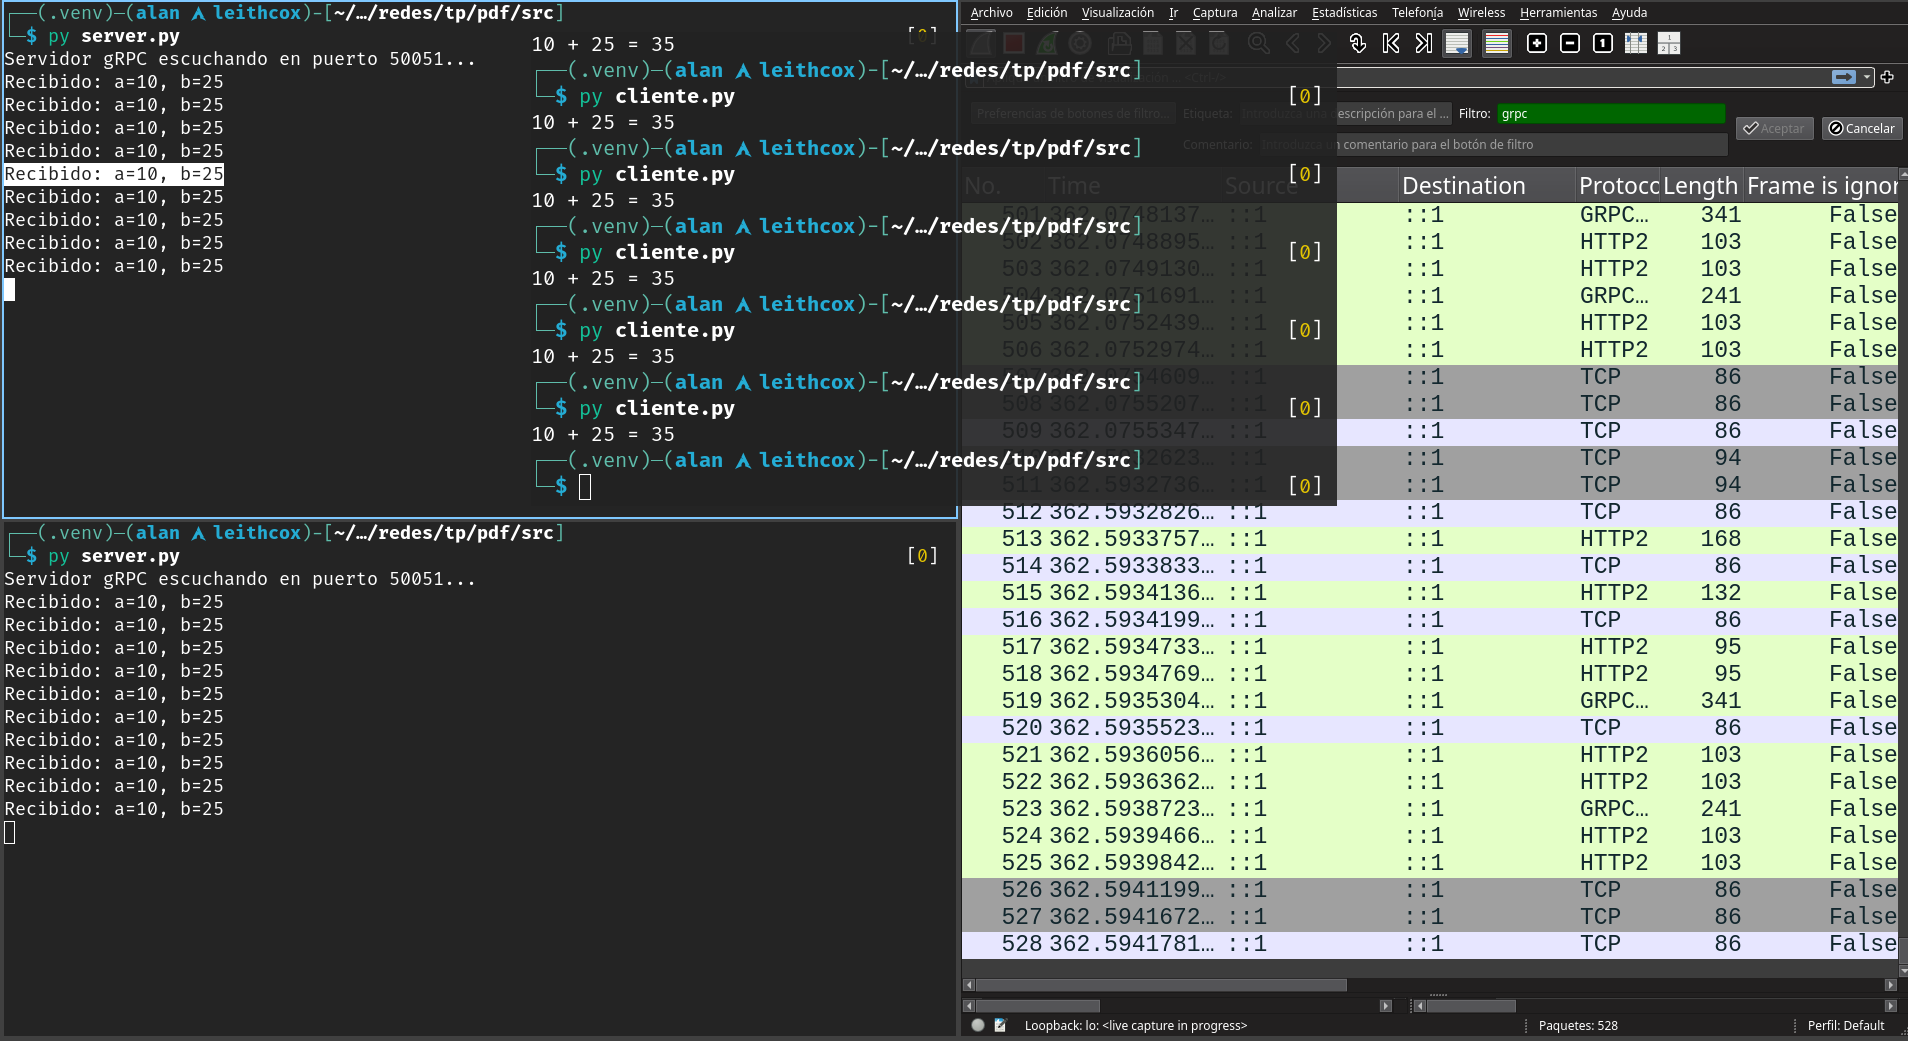
\includegraphics[width=.8 \textwidth]{3d}
                \caption{}
                \label{fig:3d}
            \end{figure}

            Al crear el servidor asignando el mismo puerto \texttt{server.add\_insecure\_port('[::1]:50051')}, se utiliza el parámetro SO\_REUSEPORT, que permite que varios procesos utilicen el mismo puerto. % REDACTAR MEJOR
            El kernel distribuye la carga por lo que, no siempre el mismo servidor atenderá la petición del mismo cliente.
            
            No se observa tráfico estpecífico entre el cliente y los distintos servidores.
            Es indistinto si hay uno como si hay varios.

            argumentar argumentar argumentar argumentar argumentar argumentar argumentar argumentar argumentar argumentar argumentar argumentar argumentar argumentar argumentar argumentar argumentar argumentar argumentar argumentar argumentar argumentar argumentar argumentar argumentar argumentar argumentar argumentar argumentar argumentar argumentar argumentar argumentar argumentar argumentar argumentar argumentar argumentar argumentar argumentar 
    \end{enumerate}
\end{problem}

\end{document}
